\documentclass{beamer}
\usepackage{lmodern}
\beamertemplatenavigationsymbolsempty

\title{SIAM-IMA Etymo workshop - Keyword Extraction}
\author{Steven Elsworth}
\date{June 13, 2018}

\begin{document}
\maketitle

\begin{frame}
 \frametitle{\centerline{Keyword Extraction}}
\begin{figure}[h]
\centering
\begin{minipage}{0.45\textwidth}
\centering
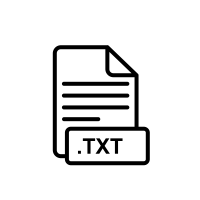
\includegraphics[width=0.7\textwidth]{img/txt}
\end{minipage}
\begin{minipage}{0.45\textwidth}
\centering

\includegraphics[width=1.2\textwidth]{img/keywords}
\end{minipage}
\end{figure}

\begin{figure}[h]
\begin{minipage}{0.45\textwidth}
\centering
Example text
\end{minipage}
\begin{minipage}{0.45\textwidth}
\centering
List of keywords
\end{minipage}
\end{figure}
\end{frame}

\begin{frame}
\frametitle{Example Data}
\textbf{Title:} Compatibility of systems of linear constraints over the set of natural numbers
\vspace{0.1in}

\textbf{Abstract:} Criteria of compatibility of a system of linear Diophantine equations, strict inequations, and nonstrict inequations are considered. Upper bounds for components of a minimal set of solutions and algorithms of construction of minimal generating sets of solutions for all types of systems are given. These criteria and the corresponding algorithms for constructing a minimal supporting set of solutions can be used in solving all the considered types of systems and systems of mixed types.

\textbf{Manually assigned keywords:}
linear constraints, set of natural numbers, linear Diophantine equations, strict inequations, nonstrict inequations, upper bounds, minimal generating sets
\end{frame}

%\begin{frame}
%\frametitle{Previous Approaches}
%\begin{itemize}
%\item Machine Learning
%\vspace{0.5in}
%\item TFIDF
%\vspace{0.5in}
%\item RAKE
%\vspace{0.5in}
%\item Graph Based Approaches
%\end{itemize}
%\end{frame}

\begin{frame}
\frametitle{Neural nets}
We do not have the training data. 

\vspace{0.2in}

\begin{itemize}
\item \url{https://www.worldcat.org}

\item \url{https://www.sciencedirect.com/science/article/pii/S0957417417308473}

\item \url{https://www.worldscientific.com/doi/abs/10.1142/S0218213004001466}

\item \url{https://epubs.siam.org/doi/abs/10.1137/17M1119901}
\end{itemize}

\end{frame}

\begin{frame}
\frametitle{TFIDF: Term Frequency, Inverse Document Frequency}

\includegraphics[width= \textwidth]{img/tfidf}
\vspace{0.5cm}
Published in 1972, led to TF-IDF .
\vspace{0.5cm}
\[
TF(t) = \frac{\text{Number of times term t appears in a document}}{\text{Total number of terms in the document}}
\]
\[
IDF(t) = \log \left( \frac{\text{Total number of documents}}{{\text{Number of documents containing term t}}} \right).
\]
\[
Value = TF * IDF
\]
\end{frame}

\begin{frame}
\frametitle{TFIDF Example}
\url{http://scikit-learn.org/stable/modules/generated/sklearn.feature_extraction.text.TfidfVectorizer.html}

\vspace{0.1in}
\begin{itemize}
\item lowercase
\item stopwords
\item n-gram range 
\item idf (smoothing)
\item document frequency range
\end{itemize}

'systems' : $\frac{4}{74\log (1)}$, , 'solutions' : $\frac{4}{74\log (1)}$, 'minimal' : $\frac{4}{74\log (1)}$, 'types' : $\frac{4}{74\log (1)}$, 'considered' : $\frac{3}{74\log (1)}$, 'set', : $\frac{3}{74\log (1)}$, 'set solutions' : $\frac{3}{74\log (1)}$, ...

\end{frame}

\begin{frame}
\frametitle{RAKE: Rapid Automatic Keyword Extraction}
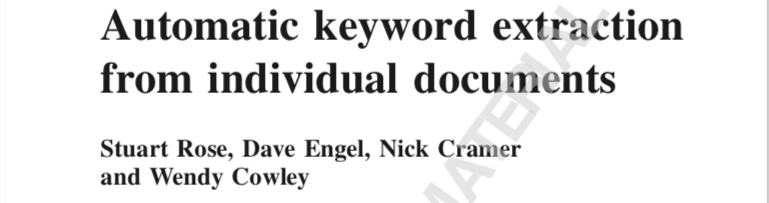
\includegraphics[width= \textwidth]{img/RAKE}
\vspace{1cm}
'An unsupervised, domain-independent, and language-independent method for extracting keywords from individual documents'
\vspace{0.5cm}

'The input parameters for RAKE comprise a list of stop words, a set of phrase delimiters, and a set of word delimiters.'
\end{frame}

\begin{frame}
\frametitle{RAKE Example}
\begin{itemize}
\item \textbf{Document:} 'A matrix is a rectangular array of numbers, symbols, or expressions, arranged in rows and columns.'
\vspace{0.3cm}
\item \textbf{Stop words:} Fox, Christopher. "A stop list for general text." ACM SIGIR Forum. Vol. 24. No. 1-2. ACM, 1989.
\vspace{0.3cm}
Example = ' a, about, above, across, after, again, against, all, almost, alone, along, already, also, although, always, among, an, ...'
\item \textbf{Phrase delimiters:} '.', ',', '!', ':', ';'
\vspace{0.3cm}
\item \textbf{Word delimiters:} ' ', '  ', '   ', '    ', '     ', ...
\end{itemize}
\end{frame}

\begin{frame}
\frametitle{RAKE: Extracted Keywords}

\url{https://github.com/zelandiya/RAKE-tutorial}

\vspace{0.1in}
compatibility, systems, linear constraints, set, natural numbers, criteria, compatibility, system, linear diophantine equations, strict inequations, nonstrict inequations, upper bounds, components, minimal set, solutions, algorithms, minimal generating sets, solutions, systems, criteria, corresponding algorithms, constructing, minimal supporting set, solving, systems, systems
\pause
\[
\text{score} = \frac{\texttt{deg}(w)}{\texttt{freq}(w)}
\]
\pause
minimal generating sets (8.7), linear diophantine equations (8.5), minimal supporting set (7.7), minimal set (4.7), linear constraints (4.5), natural numbers (4), strict inequations (4), nonstrict inequations (4), upper bounds (4), corresponding algorithms (3.5), set (2), algorithms (1.5), compatibility (1), systems (1), criteria (1), system (1), components (1),constructing (1), solving (1)
\end{frame}

\begin{frame}
\frametitle{Graph Based Approach}
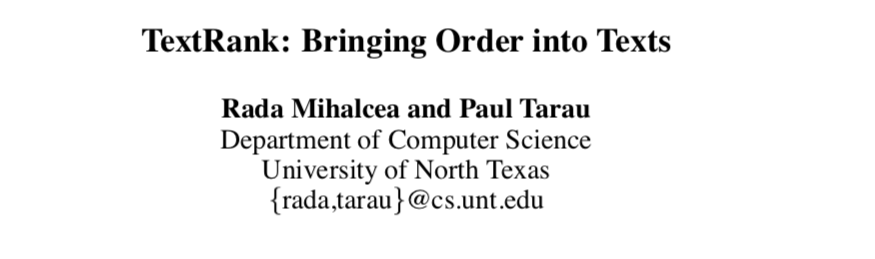
\includegraphics[width= \textwidth]{img/textrank}

\begin{enumerate}
\item Identify text units that best define the task at hand, and add them as vertices in the graph.
\item Identify relations that connect such text units, and use these relations to draw edges between vertices in the graph. Edges can be directed or undirected, weighted or unweighted.
\item Graph-based ranking algorithm.
\item Sort vertices based on their final score. Use the values attached to each vertex for ranking/selection decisions.
\end{enumerate}
\end{frame}

\begin{frame}
\frametitle{Graph Based Approach Example}

\url{https://github.com/davidadamojr/TextRank}

\vspace{0.1in}

Construct co-occurrence relation, two vertices are connected if the words appear within a window of maximum words, where can be set anywhere from 2 to 10 words.
\begin{center}
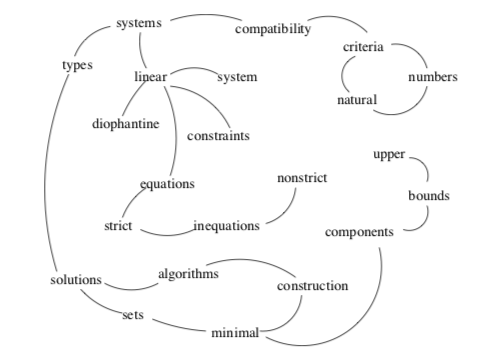
\includegraphics[scale = 0.3]{img/graph}
\end{center}
Apply graph ranking algorithm:

numbers (1.46), inequations (1.45), linear (1.29), diophantine (1.28), upper (0.99), bounds (0.99), strict (0.77), ....

\vspace{0.1in}
Postprocessing.
\end{frame}


\begin{frame}
\frametitle{Literature Review}
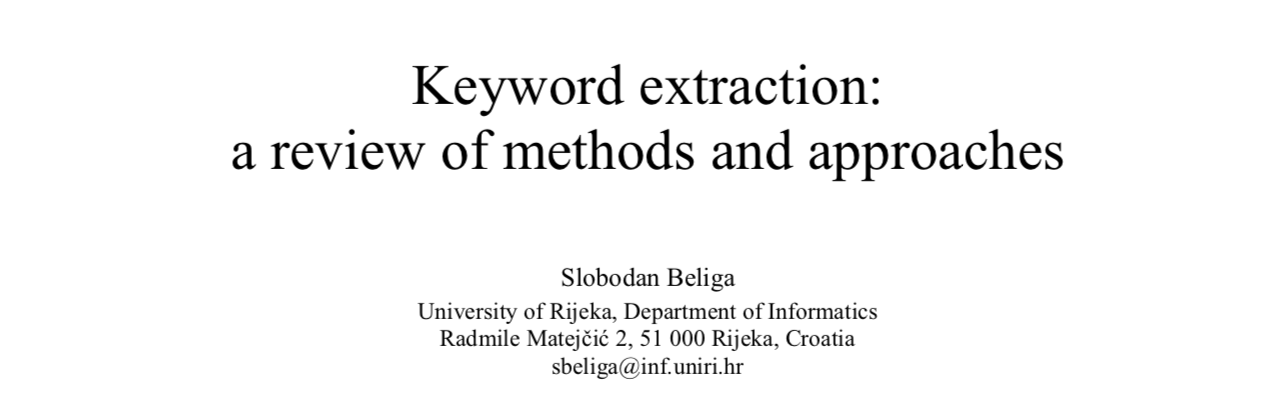
\includegraphics[width= 1\textwidth]{img/lit_review}
\vspace{0.2in}
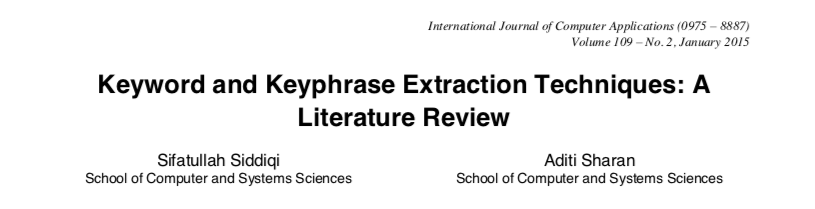
\includegraphics[width= 1\textwidth]{img/lit_review2}
\end{frame}

\end{document}
